\documentclass{article}
\usepackage[english]{babel}
\usepackage{url}
\usepackage{bytefield}
\usepackage{verbatim}
\usepackage{listings}
\usepackage{tikz}
\usetikzlibrary{calc}
\usetikzlibrary{arrows.meta}




\newcommand{\queue}[2]{%
	\begin{scope}[shift={#1},scale=#2]%
		\draw[fill=white,draw=black] (-0.5,0) rectangle (0.5,-4);%
		\foreach \i in {-1,-2,-3}%
		\draw (-0.5,\i) -- (0.5,\i);%
	\end{scope}%
}
\newcommand{\multiplexerpic}{
	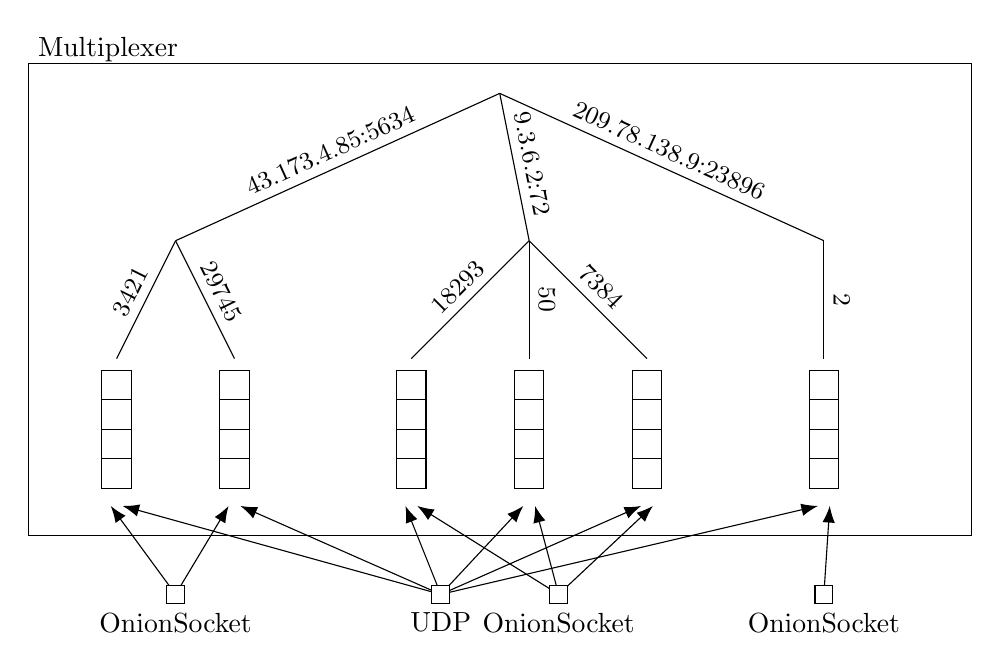
\begin{tikzpicture}[scale=\textwidth/16.2cm]
	\draw[draw=black] (0,0) rectangle (16,8);
	\node[anchor=west] at (0,8.25) {Multiplexer};
	\coordinate (root) at (8,7.5);
	\coordinate (peer1) at (2.5,5);
	\coordinate (peer2) at (8.5,5);
	\coordinate (peer3) at (13.5,5);
	\coordinate (conn11) at (1.5,3);
	\coordinate (conn12) at (3.5,3);
	\coordinate (conn21) at (6.5,3);
	\coordinate (conn22) at (8.5,3);
	\coordinate (conn23) at (10.5,3);
	\coordinate (conn31) at (13.5,3);
	\coordinate (onionsocket1) at (2.5,-1);
	\coordinate (onionsocket2) at (9,-1);
	\coordinate (onionsocket3) at (13.5,-1);
	\coordinate (udp) at (7,-1);
	\draw (root) -- node[sloped,anchor=center,above] {\small{}43.173.4.85:5634\normalsize} (peer1);
	\draw (root) -- node[sloped,anchor=center,above] {\small{}9.3.6.2:72\normalsize} (peer2);
	\draw (root) -- node[sloped,anchor=center,above] {\small{}209.78.138.9:23896\normalsize} (peer3);
	\draw (peer1) -- node[sloped,anchor=center,above] {\small{}3421\normalsize} (conn11);
	\draw (peer1) -- node[sloped,anchor=center,above] {\small{}29745\normalsize} (conn12);
	\draw (peer2) -- node[sloped,anchor=center,above] {\small{}18293\normalsize} (conn21);
	\draw (peer2) -- node[sloped,anchor=center,above] {\small{}50\normalsize} (conn22);
	\draw (peer2) -- node[sloped,anchor=center,above] {\small{}7384\normalsize} (conn23);
	\draw (peer3) -- node[sloped,anchor=center,above] {\small{}2\normalsize} (conn31);
	\queue{($ (conn11) + (0,-0.2) $)}{0.5}
	\queue{($ (conn12) + (0,-0.2) $)}{0.5}
	\queue{($ (conn21) + (0,-0.2) $)}{0.5}
	\queue{($ (conn22) + (0,-0.2) $)}{0.5}
	\queue{($ (conn23) + (0,-0.2) $)}{0.5}
	\queue{($ (conn31) + (0,-0.2) $)}{0.5}
	\draw[-{Latex[length=6pt]}] (onionsocket1) --  ($ (conn11) + (-0.1,-2.5) $);
	\draw[-{Latex[length=6pt]}] (onionsocket1) -- ($ (conn12) + (-0.1,-2.5) $);
	\draw[-{Latex[length=6pt]}] (onionsocket2) --  ($ (conn21) + (0.1,-2.5) $);
	\draw[-{Latex[length=6pt]}] (onionsocket2) -- ($ (conn22) + (0.1,-2.5) $);
	\draw[-{Latex[length=6pt]}] (onionsocket2) -- ($ (conn23) + (0.1,-2.5) $);
	\draw[-{Latex[length=6pt]}] (onionsocket3) -- ($ (conn31) + (0.1,-2.5) $);
	\draw[-{Latex[length=6pt]}] (udp) --  ($ (conn11) + (0.1,-2.5) $);
	\draw[-{Latex[length=6pt]}] (udp) -- ($ (conn12) + (0.1,-2.5) $);
	\draw[-{Latex[length=6pt]}] (udp) --  ($ (conn21) + (-0.1,-2.5) $);
	\draw[-{Latex[length=6pt]}] (udp) -- ($ (conn22) + (-0.1,-2.5) $);
	\draw[-{Latex[length=6pt]}] (udp) -- ($ (conn23) + (-0.1,-2.5) $);
	\draw[-{Latex[length=6pt]}] (udp) -- ($ (conn31) + (-0.1,-2.5) $);
	\draw[fill=white,draw=black] ($ (onionsocket1) + (-0.15,-0.15) $)  rectangle ($ (onionsocket1) + (0.15,0.15) $);
	\draw[fill=white,draw=black] ($ (onionsocket2) + (-0.15,-0.15) $)  rectangle ($ (onionsocket2) + (0.15,0.15) $);
	\draw[fill=white,draw=black] ($ (onionsocket3) + (-0.15,-0.15) $)  rectangle ($ (onionsocket3) + (0.15,0.15) $);
	\draw[fill=white,draw=black] ($ (udp) + (-0.15,-0.15) $)  rectangle ($ (udp) + (0.15,0.15) $);
	\node[anchor=north] at ($ (onionsocket1) + (0,-0.15) $) {OnionSocket};
	\node[anchor=north] at ($ (onionsocket2) + (0,-0.15) $) {OnionSocket};
	\node[anchor=north] at ($ (onionsocket3) + (0,-0.15) $) {OnionSocket};
	\node[anchor=north] at ($ (udp) + (0,-0.15) $) {UDP};
	\end{tikzpicture} \\
	
}





\begin{document}
\title{\Huge Final Report \normalsize}
\date{\today}
\author{\LARGE 16 Onions \normalsize \\[5pt] Charlie Groh \hspace{20pt} Josef Stark}
\maketitle
{\let\thefootnote\relax\footnotetext{This work is licensed under the Creative
Commons Attribution-ShareAlike 4.0 International License. To view a copy of
this license, visit http://creativecommons.org/licenses/by-sa/4.0/ or send a
letter to Creative Commons, PO Box 1866, Mountain View, CA 94042, USA.}}

\section{General}
We are the team ``16 Onions'' consisting of Charlie Groh and Josef Stark,
and our goal is to develop a prototype implementation of the Onion module.

\section{Application Internals}
In this section we will describe the general structure of the application, the network protocol we implemented, as well as an overview over how the source code is organized.

\subsection{Network Protocols}
For the communication between distinct onion instances we decided to use both TCP and UDP as underlying protocols in order to avoid reinventing the wheel, since they both fulfill the respective requirements perfectly.

Control messages, i.e. messages for authentication, tunnel construction, tunnel destruction and heartbeat are transferred and forwarded over TCP, because for those messages it is very important that they actually arrive or that we get feedback if one of those messages could not be delivered to the target, so we can react in an appropriate manner---e.g. assume that the corresponding node went down and construct an alternative route. TCP satisfies these requirements as it acknowledges the reception of messages, resends messages if necessary and reports a failure if a message still didn't provoke an acknowledgement after a few retries. If we used UDP instead, we would have had to re-implement all of these features by hand. 

User data messages, i.e. messages containing VoIP and cover data, are transferred and forwarded over UDP, since for those a short delay is a requirement which UDP can satisfy. UDP is packet based and does not acknowledge the arrival of packets at all, so the lower delay that this causes comes at the price of possibly losing some packets which are not resent and therefore never reach their target, without the sender being informed about the loss. This is acceptable for VoIP and cover data.

Other modules can use the onion module only to send user data messages (UDP), while control messages are exclusively used internally for tunnel management tasks.

\subsubsection{Layer 0: Network Abstraction Layer}

At the lowest level of our application lies the so-called multiplexer, which abstracts away low-level protocol details of the underlay connections and offers a clean interface for message interchange between nodes via logical overlay connections. The core tunnel mechanisms exclusively use this interface. The main tasks of the multiplexer are:
\begin{itemize}
	\item Establishing and terminating control data channels to other peers using TCP
	\item Establishing and terminating user data channels to other peers using UDP
	\item Padding/Unpadding messages to/from a fixed, configurable size while offering transport functionality of variable-sized payload
	\item Correctly assigning and relating incoming and outgoing messages to the tunnel they belong to
\end{itemize}
Upon receiving the request to connect to a certain peer, the multiplexer first establishes a TCP connection to that peer for transporting control data and then immediately sends a packet to that peer containing the UDP port on which it is listening for user data: \\

	\begin{bytefield}[bitwidth=1.0em]{32}
		\bitheader{0,7,8,15} \\
		\bitbox{16}{UDP listening port number} \\
	\end{bytefield} \\
(TCP message)

This is the only message type that is exchanged on its own. After it has been sent, messages are only sent upon request of the core tunnel mechanism. They can be transmitted over TCP or UDP, which is controlled by a flag of the corresponding function. They have the following structure:

	\begin{bytefield}[bitwidth=1.0em]{32}
		\bitheader{0,7,8,15,16,23,24,31} \\
		& \bitbox{16}{payload length} 
		& \bitbox{16}{tunnel ID} \\
		\bitbox[lrt]{32}{payload} \\
		\skippedwords \\				
		\bitbox[lrt]{32}{padding} \\
		\skippedwords \\
		\wordbox[blr]{1}{}
	\end{bytefield} \\
(TCP or UDP message) \\


Whenever a previously unknown peer---that is, a host with a source address-port combination, which did not communicate with the peer previously---connects (via TCP) to the peer, the multiplexer assigns an ID to that connection and creates a message queue for it. All incoming messages from the underlying connections are assigned and put into the respective queue belonging to the connection: Messages from \texttt{OnionSocket}, which are basically TCP messages, as well as UDP messages, whose filtering would otherwise need to be done by hand, since UDP is by nature connectionless. The queues, which are essentially the logical overlay connections exported by the multiplexer, can be accessed by their previously assigned ID to read and write TCP and UDP packets---or rather control and data messages, represented by the \texttt{OnionMessage} class. Even though there are no separate queues for TCP and UDP packets of a connection, their type can be determined to be control or data message via \texttt{type} field. 
\multiplexerpic{}
New connections are signaled by calling the \texttt{newConnection()} method, where almost all higher-level (Layer 1) messaging is done.

\subsubsection{Layer 1: Tunnel Management Layer}
The core tunnel mechanisms build upon the network abstraction layer provided by the multiplexer and use its interface to access the logical overlay connections and exchange messages. Those messages, which will be described in this section are thus free of metadata and padding from Layer 0. This information is added/removed and generally handled transparently by the multiplexer.

This section lists each message type and their exact structure used during all the phases of a tunnel lifespan. For the sake of readability, we will refer to the initiator of a connection as "peer A" and to the other node as "peer B".

\begin{itemize}
	\item Handshake 1 \\

		\begin{bytefield}[bitwidth=1.0em]{32}
			\bitheader{0,7,8,15,16,23,24,31} \\
			& \bitbox{8}{MAGIC SEQ}
			& \bitbox{8}{VERSION}
			& \bitbox[lrt]{16}{} \\
			\bitbox[lr]{32}{Handshake 1} \\
			\skippedwords \\	
			\wordbox[blr]{1}{}			
		\end{bytefield} \\
		(TCP message)
		
		This message is sent from peer A to initiate the authentication process. MAGIC SEQ is a bit sequence identifying the connection initiator as onion peer; VERSION contains the P2P protocol version. Handshake 1 is obtained from the ONION AUTH module of peer A and forwarded to peer B via this message, where it is passed to the local ONION AUTH module---given that it is actually a onion node, MAGIC SEQ matches and VERSION is compatible.
		
	\item Handshake 2 \\

		\begin{bytefield}[bitwidth=1.0em]{32}
			\bitheader{0,7,8,15,16,23,24,31} \\
			\bitbox[lrt]{32}{Handshake 2} \\
			\skippedwords \\				
			\wordbox[blr]{1}{}
		\end{bytefield} \\
		(TCP message)
		
		After having processed Handshake 1, peer B obtains Handshake 2 from its ONION AUTH module---given that the Handshake was valid. It then sends this Handshake 2 back to peer A. ONION AUTH of peer A now checks the received Handshake for validity. If positive, the handshake is further processed and an encrypted connection between peer A and peer B has been established. In any other case---peer A received an invalid handshake or no answer at all and timed out---the authentication is aborted and adequate measures are to be taken, e.g. selecting a different node and starting over the procedure.
	
	\item Tunnel building/expansion request \\
	
		\begin{bytefield}[bitwidth=1.0em]{32}
			\bitheader{0,7,8,15,16,23,24,31} \\
			& \bitbox{8}{TUN BUILD}
			& \bitbox{8}{addr length}
			& \bitbox[lrt]{16}{} \\
			\bitbox[lr]{32}{IP address} \\
			\skippedwords \\	
			\bitbox[blr]{16}{}		
			& \bitbox{16}{port number}	
		\end{bytefield} \\
		(TCP message)
		
		Peer A can send this message to an authenticated peer B to instruct it to connect to another peer C, whose address is specified in this message. Upon receiving it, peer B will now forward all incoming messages between peer A and peer C, so peer A can begin authenticating with peer C over peer B.
		
	\item Incoming tunnel notification \\
			
		\begin{bytefield}[bitwidth=1.0em]{32}
			\bitheader{0,7} \\
			& \bitbox{8}{TUN INCOMING}
		\end{bytefield} \\
		(TCP message)
		
		This message is sent from peer A to the peer D at the end of the tunnel, so that peer D knows that the established tunnel ends at peer D and that the further incoming data is destined to him and must not be forwarded. After receiving this message, no more tunnel building/expansion requests can be sent to peer D.
		
	\item User data \\
	
	\begin{bytefield}[bitwidth=1.0em]{32}
		\bitheader{0,7,8,15,16,23,24,31} \\
		& \bitbox{8}{DATA}
		& \bitbox[lrt]{24}{} \\
		\bitbox[lr]{32}{payload} \\
		\skippedwords \\	
		\wordbox[blr]{1}{}
	\end{bytefield} \\
	(UDP message)
	
	Contains real user (i.e. VoIP) data, which was requested to be sent by another local module. Requires the previous reception of an incoming tunnel notification in order to be interpreted.
	
	\item User data \\
	
		\begin{bytefield}[bitwidth=1.0em]{32}
			\bitheader{0,7,8,15,16,23,24,31} \\
			& \bitbox{8}{COVER}
			& \bitbox[lrt]{24}{} \\
			\bitbox[lr]{32}{random data} \\
			\skippedwords \\	
			\wordbox[blr]{1}{}
		\end{bytefield} \\
		(UDP message)
		
		Contains cover traffic of a specified size, which was requested to be sent by the local CM/UI module. Since it contains no meaningful data, the message is discarded upon reception.
		
	\item Heartbeat \\
	
	\begin{bytefield}[bitwidth=1.0em]{32}
		\bitheader{0,7} \\
		& \bitbox{8}{HEARTBEAT}
	\end{bytefield} \\
	(UDP message)
	
	If a time-out was triggered, meaning that a peer has not received data of any kind from a certain tunnel in a predefined amount of time, it sends this message to request a sign of live from the node at the other end of the tunnel. This sign of live can be any data, but if there is currently no real user data available for being sent, it is simply cover traffic.
	Each time-out triggers the sending of such a heartbeat message and the incrementation of a retries-counter. Once a response has been received, that counter is reset to zero; if the counter exceeds five, the tunnel is presumed dead. This message (as well as cover traffic and real data) can only be sent by the two end nodes of a tunnel. An intermediate hop also counts the time-outs and disconnects from its predecessor and successor if necessary, but does not send messages on its own, it only forwards them.
\end{itemize}
	
	\subsection{Mode of Operation}
	After the application has been initialized, it accepts requests from the CM/UI to:
	\begin{itemize}
		\item Build tunnels
		\item Destroy tunnels
		\item Send data through tunnels
		\item Send cover traffic through tunnels
	\end{itemize}
	Apart from that, it listens for new incoming tunnels and data arriving through tunnels and notifies the CM/UI for any of those events. \\
	Time in the system is divided into equal intervals called rounds. New tunnels are established at the beginning of the next round and destroyed upon request. If at the beginning of a round there is not any tunnel in existence or pending to be built, the module builds a tunnel to a random destination, which is automatically destroyed at the end of the round. This kind of tunnel can only be used to send cover traffic.
	
	\subsubsection{Tunnel Construction Process}
	The class used for constructing outgoing tunnels is called \texttt{OnionConnectingSocket}. For incoming as well as intermediate tunnels (when a peer is only forwarding traffic), \texttt{OnionListenerSocket} is used. The process of constructing it is as follows:
	\begin{enumerate}
		\item An array of intermediate hops is constructed by repeatedly asking the RPS module for random peers. The amount of hops is determined in the config file. The last node is the specified target.
		\item The first unconnected node in the hop array is selected.
		\item Handshake 1 is generated and sent to the selected hop.
		\item Handshake 2 is received.
		\item Test, if there are any unconnected hops remaining in the array: 
		\begin{enumerate}
			\item If yes: A tunnel building/expansion request, containing the next hop as target, is sent to the current hop. That hop then connects to the specified target and forwards all traffic coming through that tunnel to it and vice-versa. The next unconnected node in the array is connected and the next loop iteration executed, starting at point 3.
			\item If not: The tunnel endpoint is reached, so the incoming tunnel notification is sent.
		\end{enumerate}
	\end{enumerate}
	If during this construction process an unexpected packet is received or an answer takes too long, a different intermediate peer is selected or, if the node in question is the tunnel endpoint, the construction is aborted and the failure, if required, reported to the CM/UI module.
	
	Once established, a tunnel can and will be used to transfer data-messages, heartbeats and cover-traffic. 
	
	While the CM/UI cannot explicitly send cover data over tunnels whose construction it requested, cover messages are used internally if a node needs to respond to a Heartbeat and has no real user data available to be sent.
	
	\subsubsection{Tunnel Destruction Process}
	Tearing down a tunnel happens in the reverse order of construction: The respective message is sent to all hops, starting with the tunnel node to the node which is directly connected to the initiator. Once a hop receives the message, it closes the connection to its predecessor in that tunnel. Should an error happen while sending the message

\section{Usage}
In order to use the module, a Java runtime environment (version 7 or later), as well as Apache Ant\footnote{\url{https://ant.apache.org/}} is needed on the host. The code depends on some 3rd-party libraries, but they are all included in the repository. \\
For further development of the module, Eclipse\footnote{\url{http://www.eclipse.org/}} (version 3.8 or later) with Lombok\footnote{\url{https://projectlombok.org/}} (version 1.16.16 or later) is recommended. The respective project file is included.
To use the module, the RPS and ONION AUTH modules have to be started. Also, the module has to be compiled and the class \texttt{Main} of the package \texttt{com.voidphone.onion} must be started. Those last two things can be done either via the respective GUI commands in Eclipse or via command-line interface:
\begin{lstlisting}
.../16onions$ ant clean
.../16onions$ ant build
.../16onions$ java -classpath bin:\
libs/ini4j-0.5.4.jar:\
libs/commons-cli-1.3.1.jar:\
testing/libs/bcprov-jdk15on-155.jar:\
testing/libs/lombok-1.16.16.jar \
com.voidphone.onion.Main -c <path to configuration file>
\end{lstlisting}

\subsection{Configuration}
The module needs a hostkey, which it will use to identify itself to other peers, as well as a configuration file with all the necessary options specified. The hostkey can be generated like this:
\begin{lstlisting}
openssl genrsa -out hostkey.pem 4096
\end{lstlisting} 
The configuration file needs to be in INI format. Here is how an example configuration file could look like:
\begin{lstlisting}
[onion]
hostkey = /home/p2p/hostkey.pem
api_address = 0.0.0.0:2223
listen_address = 0.0.0.0:2512
hopcount = 3
api_timeout = 2000
p2p_timeout = 2000
p2p_packetsize = 20480
roundtime = 15000
[auth]
api_address = 0.0.0.0:2023
[rps]
api_address = 0.0.0.0:2123
\end{lstlisting}
Explanation of the options:
\begin{itemize}
\item \texttt{hostkey}: Path to the hostkey
\item \texttt{api\_address} in sections \texttt{[auth]} and \texttt{[rps]}: The listening address---consisting of binding address and port---of the API interfaces of ONION AUTH and RPS modules
\item \texttt{api\_address} in section \texttt{[onion]}: The listening address---consisting of binding address and port---of the onion module API, where it will listen and respond to API requests from the CM/UI module
\item \texttt{listen\_address}: The P2P listening address---consisting of binding address and port---where the onion module will listen for new incoming tunnels from other nodes
\item \texttt{hopcount}: The amount of intermediate hops used for building outgoing tunnels. This number does not include start and end node, i.e. a hopcount of zero equals a direct connection.
\item \texttt{api\_timeout}: The API timeout in milliseconds. When waiting for a response from one of the API interfaces, the module will give up after not receiving anything in the given amount of time.
\item \texttt{p2p\_timeout}: The P2P timeout in milliseconds. If, for any given tunnel, which the local module instance is a part of, no message has been arrived, measures are taken (i.e. the sending or forwarding of a heartbeat) to ensure that it is still alive. If those measures are unsuccessful, the respective tunnel is presumed dead and torn down.
\item \texttt{p2p\_packetsize}: The size in bytes which all incoming and outgoing messages are padded/unpadded to/from by the multiplexer. This value should be moderately low in order to avoid excessive, unnecessary UDP packet loss: Even small messages are padded to the specified size, and big UDP messages are often segmented, and if even one segment does not arrive at the target, the whole packet will be discarded, even if the loss would only affect the padding. Also, it must be the same on all peers. Nonetheless, we left this as a config option, since at the same time it must be sufficiently high so that the payloads returned by ONION AUTH fit into a message and we do not know what their size is, since our module should run with any ONION AUTH implementation.
\item \texttt{roundtime}: The roundtime in milliseconds
\end{itemize}
The path to the config file is passed to the module as parameter, as explained before.
	
\subsection{Testsuite}
The module contains a testsuite that tests artificial and real world situations. The testsuite is
located in the package \texttt{com.voidphone.testing}. The class \texttt{Testing} is a unit test
that tests the module for API conformance and some basic functionality like building a tunnel
between two hops. The class \texttt{Test} launches multiple hops and tries to build multiple
tunnels between them. When the test terminates, it will print the number of successful calls.

In order to avoid stale files, the testsuite will delete generated config files in \texttt{tmp/}
after executing the test. If you want to keep them, you must set \texttt{deleteConfigAfterTest}
to \texttt{false} in the \texttt{Helper} class. To prevent stale open ports, every started process
is killed after usage. In addition, every test is terminated after at most two minutes.
Unfortunately, we were not able to add satisfying support for the \texttt{SecurityHelper} class in
the \texttt{testing}-module. So it may be necessary to hardcode the keystore path in the
\texttt{propertiesPath} variable.
The testing module does not need to be provided with hostkeys and configuration files, since it generates them on-the-fly by itself.

To run the tests, everything has to be built and the classes \texttt{Testing} and \texttt{Test} run. This can all be done via the respective Eclipse GUI commands or else via command-line interface:

\begin{lstlisting}
.../16onions$ ant clean
.../16onions$ ant build

.../16onions$ java -classpath bin:\
libs/ini4j-0.5.4.jar:\
libs/commons-cli-1.3.1.jar:\
testing/libs/junit-4.12.jar:\
testing/libs/test/hamcrest-core-1.3.jar:\
testing/libs/bcprov-jdk15on-155.jar:\
testing/libs/lombok-1.16.16.jar \
org.junit.runner.JUnitCore com.voidphone.testing.Testing

.../16onions$ java -classpath bin:\
libs/ini4j-0.5.4.jar:\
libs/commons-cli-1.3.1.jar:\
testing/libs/junit-4.12.jar:\
testing/libs/test/hamcrest-core-1.3.jar:\
testing/libs/bcprov-jdk15on-155.jar:\
testing/libs/lombok-1.16.16.jar \
org.junit.runner.JUnitCore com.voidphone.testing.Test
\end{lstlisting}

\section{Bugs and Limitations}

\section{Project Work}
Although there are still some bugs in our module, we consider the project as successful.

\subsection{Work Distribution}

\subsection{Spent Effort}
Since we mostly worked on the project at the same time, the effort spent by each individual is
almost identical. On average, every team member spent around three hours per week for the project.

\noindent


\end{document}
\grid
